\section{test}

% Set the overall layout of the tree
\tikzstyle{level 1}=[level distance=3.5cm, sibling distance=3.5cm]
\tikzstyle{level 2}=[level distance=3.5cm, sibling distance=2cm]

% Define styles for bags and leafs
\tikzstyle{bag} = [text width=4em, text centered]
\tikzstyle{end} = [circle, minimum width=3pt,fill, inner sep=0pt]

% The sloped option gives rotated edge labels. Personally
% I find sloped labels a bit difficult to read. Remove the sloped options
% to get horizontal labels. 
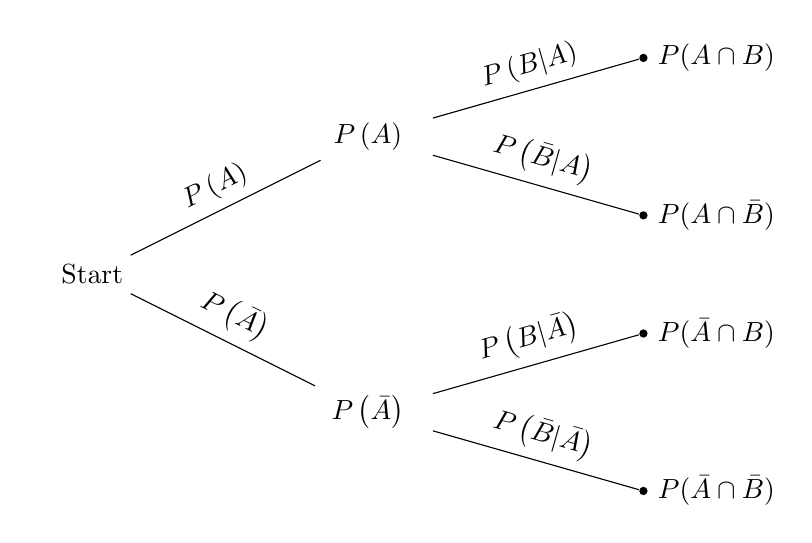
\begin{tikzpicture}[grow=right, sloped]
\node[bag] {Start}
    child {
        node[bag] {$P \left(\bar{A} \right)$}        
            child {
                node[end, label=right:
                    {$P(\bar{A}\cap \bar{B})$}] {}
                edge from parent
                node[above] {$P \left(\bar{B} \vert \bar{A} \right)$}
                %node[below]  {$\frac{4}{9}$}
            }
            child {
                node[end, label=right:
                    {$P(\bar{A}\cap B)$}] {}
                edge from parent
                node[above] {$P \left(B \vert \bar{A} \right)$}
                %node[below]  {$\frac{5}{9}$}
            }
            edge from parent 
            node[above] {$P \left(\bar{A} \right)$}
            %node[below]  {$\frac{4}{7}$}
    }
    child {
        node[bag] {$P \left(A \right)$}        
        child {
                node[end, label=right:
                    {$P(A \cap \bar{B})$}] {}
                edge from parent
                node[above] {$P \left(\bar{B} \vert A \right)$}
                %node[below]  {$\frac{3}{9}$}
            }
            child {
                node[end, label=right:
                    {$P(A\cap B)$}] {}
                edge from parent
                node[above] {$P \left(B \vert A \right)$}
                %node[below]  {$\frac{6}{9}$}
            }
        edge from parent         
            node[above] {$P \left(A \right)$}
            %node[below]  {$\frac{3}{7}$}
    };
\end{tikzpicture}